\VerdierPhysicalPageAnchor{0055}%
\VerdierSemanticAnchor{ch1-1-5-4-eq4}
From the foregoing, we know that the property $P(\lambda,\mu)$ holds
in the following cases:

\begin{equation}
  \begin{gathered}
    \lambda\ \text{and}\ \mu\in\mathbb Z^{n-1},\\
    \lambda\ \text{and}\ \mu\in\mathbb Z e_n,\\
    \lambda\in\mathbb Z^{n-1}\ \text{and}\ \mu\in\mathbb Z e_n,\\
    \lambda\in\mathbb Z e_n\ \text{and}\ \mu\in\mathbb Z^{n-1}.
  \end{gathered}
  \tag{1.5.4.4}
\end{equation}

Moreover, by (1.5.5), we have:

\VerdierSemanticAnchor{ch1-1-5-4-eq5}
\begin{quote}
  \noindent\textup{(1.5.4.5)}\quad
  \emph{If three of the properties $P(\mu,\nu)$,
  $P(\lambda+\mu,\nu)$, $P(\lambda,\mu+\nu)$, $P(\lambda,\mu)$
  are true, then so is the fourth.}
\end{quote}

\VerdierSemanticAnchor{ch1-1-5-4-conclusion}
It follows that the property $P(\lambda,\mu)$ is true for every pair
$\lambda,\mu\in\mathbb Z^n$, which completes the proof of
Proposition (1.5.2).

\VerdierSemanticAnchor{ch1-1-5-5}
\noindent\textbf{Diagram 1.5.5.}\quad
We propose to prove assertion (1.5.4.5). Let $D(\lambda,\mu)$ denote
the diagram $\textup{(1.5.4.1)}_{\lambda,\mu}$. The proof of
(1.5.4.5) is based on consideration of the following diagram, which,
for simplicity, we write in the case where the transition isomorphisms
$c$ and $c'$ are identity morphisms, \emph{i.e.} where the group
$\mathbb Z^n$ acts strictly on the categories $\mathcal C$ and
$\mathcal C'$:

\VerdierSemanticAnchor{ch1-1-5-5-tetrahedron}
\begin{center}
  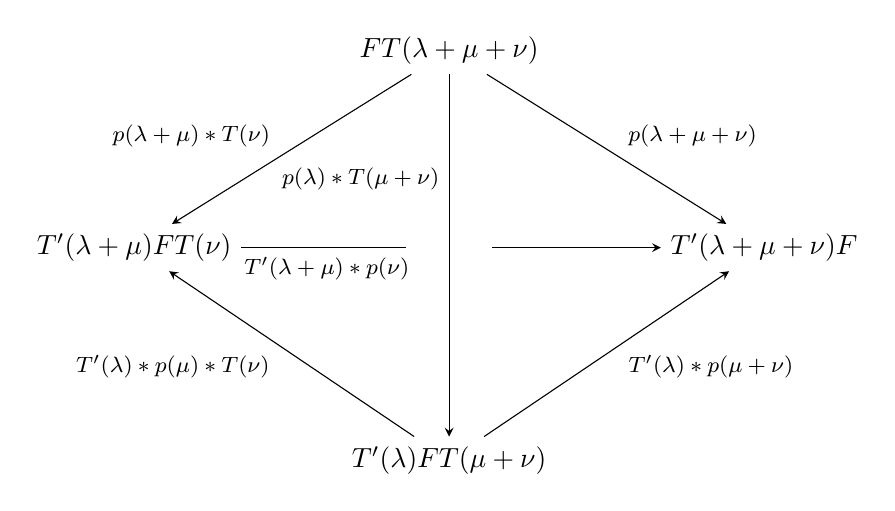
\begin{tikzpicture}[x=1cm,y=1cm,>=stealth]
    \node (a) at (0,3.2) {$FT(\lambda+\mu+\nu)$};
    \node (b) at (-4,0.7) {$T'(\lambda+\mu)FT(\nu)$};
    \node (c) at (4,0.7) {$T'(\lambda+\mu+\nu)F$};
    \node (d) at (0,-2.0) {$T'(\lambda)FT(\mu+\nu)$};
    \draw[->] (a) -- node[above left,pos=.55,font=\footnotesize]
      {$p(\lambda+\mu)*T(\nu)$} (b);
    \draw[->] (a) -- node[above right,pos=.55,font=\footnotesize]
      {$p(\lambda+\mu+\nu)$} (c);
    \draw[->] (a) -- node[left,pos=.29,font=\footnotesize]
      {$p(\lambda)*T(\mu+\nu)$} (d);
    \coordinate (bc-left) at (-0.55,0.7);
    \coordinate (bc-right) at (0.55,0.7);
    \draw (b) -- node[below,pos=.52,font=\footnotesize]
      {$T'(\lambda+\mu)*p(\nu)$} (bc-left);
    \draw[->] (bc-right) -- (c);
    \draw[->] (d) -- node[below left,pos=.55,font=\footnotesize]
      {$T'(\lambda)*p(\mu)*T(\nu)$} (b);
    \draw[->] (d) -- node[below right,pos=.55,font=\footnotesize]
      {$T'(\lambda)*p(\mu+\nu)$} (c);
  \end{tikzpicture}
\end{center}

\VerdierSemanticAnchor{ch1-1-5-5-faces}
This diagram has the form of a tetrahedron whose four faces are,
respectively, the diagrams $D(\lambda,\mu+\nu)$,
$D(\lambda+\mu,\nu)$, $D(\lambda,\mu)T(\nu)$, and
$T'(\lambda)D(\mu,\nu)$. The proof of (1.5.4.5) then proceeds by
considering the four possible cases and using the cocycle relation.

\VerdierSemanticAnchor{ch1-1-5-5-reduction}
In the general case, the diagram that must be introduced is somewhat
more complicated, but by using identities (1.2.1.3), the argument
reduces to the one sketched above. To obtain the proof of (1.5.3.5),
we use the same diagram with
\[
  \lambda=qe_1,\qquad \mu=q'e_1,\qquad \nu=q''e_1.
\]
